\documentclass[UTF8]{ctexart}

\usepackage{listings}
\usepackage{color,xcolor} 
\usepackage{colortbl}
\usepackage{graphicx}
\usepackage{booktabs} %绘制表格
\usepackage{caption2} %标题居中
\usepackage{geometry}
\usepackage{array}
\usepackage{amsmath}
\usepackage{subfigure} 
\usepackage{longtable}
\usepackage{abstract}
\usepackage{multirow}
\usepackage{enumerate}
\usepackage{float}
\usepackage{table}
%伪代码
\usepackage{algorithm}
\usepackage{algpseudocode}
\usepackage{amsmath}
\renewcommand{\algorithmicrequire}{\textbf{输入:}}  % Use Input in the format of Algorithm
\renewcommand{\algorithmicensure}{\textbf{过程:}} % Use Output in the format of Algorithm


%附录代码
\usepackage{listings}
\usepackage{xcolor}
\lstset{
    numbers=left, 
    numberstyle= \tiny, 
    keywordstyle= \color{ blue!70},
    commentstyle= \color{red!50!green!50!blue!50}, 
    frame=shadowbox, % 阴影效果
    rulesepcolor= \color{ red!20!green!20!blue!20} ,
    escapeinside=``, % 英文分号中可写入中文
    xleftmargin=2em,xrightmargin=2em, aboveskip=1em,
    framexleftmargin=2em
} 

\pagestyle{plain} %页眉消失

\geometry{a4paper,left=2.5cm,right=2.5cm,top=2.5cm,bottom=2.5cm}%设置页面尺寸
\lstset{
		numbers=left, %设置行号位置
		numberstyle=\tiny, %设置行号大小	
		keywordstyle=\color{blue}, %设置关键字颜色
		commentstyle=\color[cmyk]{1,0,1,0}, %设置注释颜色
		escapeinside=``, %逃逸字符(1左面的键),用于显示中文
		breaklines, %自动折行
		extendedchars=false, %解决代码跨页时,章节标题,页眉等汉字不显示的问题
		xleftmargin=1em,xrightmargin=1em, aboveskip=1em, %设置边距
		tabsize=4, %设置tab空格数
		showspaces=false %不显示空格
	}


		% \begin{figure}[!htbp]\centering
		% \includegraphics[width=1\textwidth]{img} % 图片相对位置
		% \label{fig:figure 0} % 图片标签
		% \end{figure}


\title{基于集成学习和多目标规划的中小微企业信贷决策}
\date{August 29, 2022}

\begin{document}
\maketitle{}
\renewcommand{\abstractname}{\Large 摘要\\}
\begin{abstract}
	\normalsize
	

	\textbf{关键字}:

\end{abstract}


\section{问题背景与重述}
\subsection{问题背景}
在现代社会中,许多的中小企业由于规模相对较小,盈利能力和抵押能力相对有限。通常向银行借贷时,银行回考量该企业
信誉等级、企业的交易票据信息、对上下游企业影响能力以及其抗风险的能力,向条件相对稳定,实力雄厚,供应关系稳定
的企业提供贷款。银行会首先根据中小企业的实力和信誉对其信用风险进行评估,
然后根据信用风险等因素确定是否进行放贷和调整借贷策略。

\subsection{问题重述}
某银行对确定要放贷企业的贷款额度为10~100万元;年利率为4$\%$~15$\%$;贷款期限为1年。
我们需要根据实际情况和所提供的数据信息,建立数学模型研究对企业的信贷策略,解决以下问题:

1. 对有信贷记录的企业,给出该银行在年度信贷总额固定时对这些企业的信贷策略。

2. 分析没有信贷记录的企业,并给出该银行在年度信贷总额为1亿元时对这些企业的信贷策略。

3. 考虑突发因素对企业的影响。研究未有信贷记录的企业,给出该银行在年度信贷总额为1亿元时的信贷调整策略。


\section{问题分析}
本问题针对的是中小企业以及是否有信贷记录的企业,可分为有无信贷记录两类去进行分析。
需要综合考虑到企业的供应关系、交易票据信息、盈利能力、对上下游企业影响能力以及其抗风险的能力等,
需要通过对信息数据的分析提取出反应企业能力的特征值,进行数学模型的构建,在不同的情况下能够给出银行合理
的信贷策略使其利益最大化。
\subsection{问题一的分析}
本问要求对 123 家已有信贷记录企业的信贷风险进行量化分析,在信贷总额固定时,给出相应信贷策略。
需要从放贷,贷款额度,利率和期限四个方面进行考虑。
我们从对不同信誉等级的企业提供相应的贷款额度、利率与是否放贷来制定策略。
第一,从所给数据进行盈利能力、对上下游企业的影响能力、发展潜力、抗风险能力等四类进行对应的特征值提取。
第二,通过$Voting$集成学习算法,对提取出的特征进行训练,得到每个企业的违约风险值。
第三,通过信誉等级计算出每个等级的风险均值,作为该等级的违约风险指标
第四,建立多目标非线性规划模型给出银行对于不同信誉等级的企业发放的相应的贷款额度与利率,从而使得银行利益最大化。
\subsection{问题二的分析}
本问是对未有信贷记录和信誉等级的企业进行信贷分析后给出银行的信贷策略。
第一,以第一问的数据特征提取方法,通过对企业的进销项发票信息进行特征值提取,得到企业的盈利利润、增值税、发展潜力、
对上下游企业影响能力以及发票的作废比例等特征值。
第二,利用训练好的$Voting$集成学习算法进行违约风险的计算,给出的策略是当风险>0.5时不予以放贷。
第三,计算违约概率,利用$Xgboost$模型,对第一问的数据进行训练后,以第二问提取到的特征值进行训练分析,对这些企业
进行信誉等级分类。
第四,通过多目标规划模型求解银行对这些未有信贷记录企业的信贷策略。
\subsection{问题三的分析}
本文需要考虑突发事件对企业以及行业的影响,来综合考虑给出302家未有信贷记录企业的信贷策略。我们考虑的是疫情对企业
的影响,疫情带来的企业经营困难,从而会出现无力还债的违约风险情况。需要在新冠疫情的影响下来进行风险系数的计算,
给出企业的风险情况,从而调整最终的信贷策略。
第一,根据第二问所提取的特征值,细分提取出行业风险、企业状况、利润增长率、废票占比、交易数量变动等五个特征值,
一次反映疫情对企业的影响。
第二,根据最终的影响程度进行聚类分析,结合该些企业的信誉等级,建立综合评价模型,不同企业具有不同的风险系数。
在已搭建好的多规划模型又加入风险系数这一新的特征值,对最终的目标规划进行修改,求解模型。
最终给出在疫情这一突发事件的影响下对该些企业的信贷策略。

\section{模型假设}
1、对已有信贷记录的企业,信誉等级依据上一年的情况划分,若去年违约则今年不予以贷款。

2、银行所求的信贷策略目标为,所得利益最大,承受的风险最低,客户流失率最小。

3、同一信誉等价下的企业,其信贷风险一致,银行给出同等的贷款和年利率。

4、对无信贷记录的企业,需要信誉评级后才决定是否贷款

5、不考虑银行出现其他不可控的因素

6、附件中所给出的企业均为请求银行贷款的企业,并非潜在客户,不论利率多企业都不会放弃贷款。


\section{符号说明}
\begin{table}[H]
	\begin{center}
		\begin{tabular}{c|l}
			\toprule[2pt]
			\rowcolor[gray]{0.8}

			\multicolumn{1}{m{8em}}{\centering 符号} & \multicolumn{1}{m{30em}}{\centering 基本说明}        \\

			%直接用合并单元格的方法来实现自定义列宽的同时,使文字居中对齐

			\midrule[1.3pt]
			$L(t)$                                   & $XGboost$迭代的目标函数                        \\   
			$\hat{y}(t-1)_i$                         & 迭代模型预测值                      \\
			$\Omega (f_t)$                           & 正则项               \\
			$Lost(I_i)$                              & $I_i$利率下的 类企业的潜在客户流失率 \\
			$Pf(i,j)$                            	& 第$i$年第$j$月的盈利状况                 \\
			$Profit$                                 & 同年利润增长率       \\
			$V(i,j)$                                & 第$i$年第$j$月的废票率                 \\
			$Void$                                 & 废票占比增长率                     \\
			$Tra(i,j)$                                 & 第$i$年第$j$月的交易数量                \\
			$Trade$                                   & 交易数量变动率                 \\
			$Q_i$								&风险乘数 \\
			$\sigma _n$							&第$i$类企业的平均风险 \\
			$\Delta $								& 企业利润 \\                            
			\bottomrule[2pt]
		\end{tabular}
	\end{center}
\end{table}



\section{模型建立与求解}
\subsection{问题一的求解}



\subsection{问题二的求解}
	\subsubsection{数据处理}
	依据问题一的数据处理方式,进行特征值的提取,最终获取到企业利润、增值税、进销项发票作废率、是否盈亏、下属分公司
	等20个特征值,用作训练模型的处理值。需要利用训练模型进等级评估,依据附件的形式,给出A、B、C、D四个信誉等级。
	\subsubsection{违约预测}
	采用已经训练好的额$Voting$模型,运用所提取的20个特征进行预测,判断这302家无信贷记录企业的违约风险,
	判断企业是否会违约。 给出的判断标准为违约风险超过50$\%$,则表示为风险高,不予以贷款。
	通过Voting模型的计算最终得到302个违约风险中,有34家企业的违约风险超过了50$\%$,即认为会违约,银行将不会向他们提供贷款。
	\subsubsection{信誉分类}
	有信贷记录的企业是依据信誉等级来进行确定贷款是否发放,对于这些没有信誉等级的企业则需要对他们进行信誉分级。
	通过对特征值的计算,来进行分级,从而确定信贷策略。

	本文采用的是$XGboost$模型进行分类,$XGboost$具有较好的分类功能,基于Boosting型的树集成模型。
	在梯度提升决策树$GBDT$基础上扩展,能够进行多线程并行计算,通过迭代生成新树,
	即可将多个分类性能较低的弱学习器组合为一个准确率较高的强学习器。采用随机森林对字段抽样,将正则项引入损失函数中,
	从而防止模型过拟合,并降低模型计算量。

	\subsubsection{$XGboost$模型建立}
	1、设模型具有$k$个决策树:
		\begin{equation}
			\hat{y_i}=\sum_{i = 1}^{k}f_k(x_i),f_k \in F    
		\end{equation}

		其中的$F$表示的为所有映射关系集合,可以得到损失函数为:

		\begin{equation}
			L(t)=\sum_{i = 1}^{k}l[y_i,\hat{y}(t-1)_i+f_t(x_i)]+\Omega (f_t)  
		\end{equation}

		$L(t)$为迭代时的目标函数,$n$为样本数量,$I$为损失函数,$\hat{y}(t-1)_i$为迭代模型的预测值,$\Omega (f_t)$为正则项。
	
	2、对$L(t)$进行二阶泰勒展开和移除常数项操:
	\begin{equation}
		\tilde{L}(t) \cong \sum_{j=i}^T[(\sum_{i\in I_j}d_i)w_i+\frac{1}{2}(\sum_{i\in I_j}g_i+\lambda )\omega ^2_j]+\gamma N  
	\end{equation}
	上式中,$d_i$为$l$对$\hat{y}(t-1)_i$的一阶导数;$g_i$为对$\hat{y}(t-1)_i$的二阶导数,$N$为叶子节点个数,
	$I_j$为每个叶子结点上样本集合,$\omega ^2_j$为每个叶子结点分数的$L_2$模的平方,$\lambda$和$\gamma$
	则为比重系数,防止产生过拟合。

	通过建立$XGboost$模型对附件2中处理得出的20个特征值进行计算。首先先用第一问的数据进行分类
	计算其信誉等级,进行附件1的比对,得出较高的准确率,表明用来分类实为合理。通过分类发现,等级越低
	其会违约的概率就越高,其中$D$为均会违约的企业。通过与$Voting$训练模型进行比对,发现训练结果较为
	接近,证明了$XGboost$模型的有效性。

	如下为利用$XGboost$训练得出的信誉等级:
	\begin{table}[H]
		\centering
		\begin{tabular}{|l|l|l|l|l|l|l|l|}
		\hline
			企业代号 & 信誉等级 & 企业代号 & 信誉等级 & 企业代号 & 信誉等级 & 企业代号 & 信誉等级 \\ \hline
			E124 & 3 & E200 & 3 & E275 & 2 & E350 & 1 \\ \hline
			E125 & 2 & E201 & 1 & E276 & 0 & E351 & 1 \\ \hline
			E126 & 3 & E202 & 2 & E277 & 2 & E352 & 1 \\ \hline
			E127 & 3 & E203 & 0 & E278 & 1 & E353 & 2 \\ \hline
			E128 & 0 & E204 & 0 & E279 & 1 & E354 & 1 \\ \hline
			E129 & 2 & E205 & 2 & E280 & 2 & E355 & 2 \\ \hline
			E130 & 0 & E206 & 0 & E281 & 0 & E356 & 2 \\ \hline
			E131 & 2 & E207 & 2 & E282 & 2 & E357 & 2 \\ \hline
			E132 & 3 & E208 & 3 & E283 & 1 & E358 & 2 \\ \hline
			E133 & 0 & E209 & 0 & E284 & 0 & E359 & 2 \\ \hline
			E134 & 0 & E210 & 0 & E285 & 3 & E360 & 2 \\ \hline
		\end{tabular}
	\end{table}

	\begin{table}[H]
		\centering
		\begin{tabular}{|l|l|l|l|l|l|l|l|}
		\hline
			企业代号 & 信誉等级 & 企业代号 & 信誉等级 & 企业代号 & 信誉等级 & 企业代号 & 信誉等级 \\ \hline
			E134 & 0 & E210 & 0 & E285 & 3 & E360 & 2 \\ \hline
			E135 & 0 & E211 & 3 & E286 & 1 & E361 & 2 \\ \hline
			E136 & 1 & E212 & 0 & E287 & 0 & E362 & 2 \\ \hline
			E137 & 0 & E213 & 0 & E288 & 3 & E363 & 1 \\ \hline
			E138 & 0 & E214 & 1 & E289 & 0 & E364 & 1 \\ \hline
			E139 & 1 & E215 & 0 & E290 & 0 & E365 & 0 \\ \hline
			E140 & 0 & E216 & 0 & E291 & 0 & E366 & 2 \\ \hline
			E141 & 0 & E217 & 3 & E292 & 1 & E367 & 2 \\ \hline
			E142 & 0 & E218 & 2 & E293 & 2 & E368 & 2 \\ \hline
			E143 & 0 & E219 & 2 & E294 & 3 & E369 & 2 \\ \hline
			E144 & 0 & E220 & 0 & E295 & 0 & E370 & 2 \\ \hline
			E145 & 0 & E221 & 1 & E296 & 1 & E371 & 2 \\ \hline
			E146 & 1 & E222 & 0 & E297 & 2 & E372 & 2 \\ \hline
			E147 & 0 & E223 & 2 & E298 & 2 & E373 & 3 \\ \hline
			E148 & 0 & E224 & 1 & E299 & 1 & E374 & 2 \\ \hline
			E149 & 0 & E225 & 0 & E300 & 0 & E375 & 2 \\ \hline
			E150 & 0 & E226 & 1 & E301 & 0 & E376 & 2 \\ \hline
			E151 & 0 & E227 & 0 & E302 & 0 & E377 & 1 \\ \hline
			E152 & 0 & E228 & 0 & E303 & 0 & E378 & 1 \\ \hline
			E153 & 3 & E229 & 0 & E304 & 1 & E379 & 2 \\ \hline
			E154 & 1 & E230 & 1 & E305 & 2 & E380 & 2 \\ \hline
			E155 & 2 & E231 & 0 & E306 & 3 & E381 & 0 \\ \hline
			E156 & 3 & E232 & 2 & E307 & 1 & E382 & 2 \\ \hline
			E157 & 2 & E233 & 1 & E308 & 1 & E383 & 2 \\ \hline
			E158 & 1 & E234 & 0 & E309 & 3 & E384 & 3 \\ \hline
			E159 & 2 & E235 & 3 & E310 & 1 & E385 & 2 \\ \hline
			E160 & 0 & E236 & 3 & E311 & 0 & E386 & 3 \\ \hline
			E161 & 1 & E237 & 3 & E312 & 1 & E387 & 2 \\ \hline
			E162 & 0 & E238 & 2 & E313 & 0 & E388 & 2 \\ \hline
			E163 & 0 & E239 & 3 & E314 & 0 & E389 & 2 \\ \hline
			E164 & 3 & E240 & 3 & E315 & 0 & E390 & 2 \\ \hline
			E165 & 0 & E241 & 3 & E316 & 3 & E391 & 2 \\ \hline
			E166 & 0 & E242 & 3 & E317 & 1 & E392 & 1 \\ \hline
			E167 & 0 & E243 & 0 & E318 & 2 & E393 & 2 \\ \hline
			E168 & 2 & E244 & 3 & E319 & 2 & E394 & 0 \\ \hline
			E169 & 1 & E245 & 1 & E320 & 2 & E395 & 1 \\ \hline
			E170 & 0 & E246 & 0 & E321 & 1 & E396 & 1 \\ \hline
			E171 & 0 & E247 & 1 & E322 & 1 & E397 & 2 \\ \hline
			E172 & 1 & E248 & 0 & E323 & 2 & E398 & 2 \\ \hline
		\end{tabular}
	\end{table}

	\begin{table}[H]
		\centering
		\begin{tabular}{|l|l|l|l|l|l|l|l|}
		\hline
			企业代号 & 信誉等级 & 企业代号 & 信誉等级 & 企业代号 & 信誉等级 & 企业代号 & 信誉等级 \\ \hline
			E173 & 2 & E249 & 2 & E324 & 0 & E399 & 2 \\ \hline
			E174 & 1 & E250 & 0 & E325 & 1 & E400 & 2 \\ \hline
			E175 & 0 & E251 & 1 & E326 & 0 & E401 & 1 \\ \hline
			E176 & 0 & E252 & 0 & E327 & 2 & E402 & 2 \\ \hline
			E177 & 0 & E253 & 0 & E328 & 2 & E403 & 2 \\ \hline
			E178 & 1 & E254 & 2 & E329 & 2 & E404 & 3 \\ \hline
			E179 & 0 & E255 & 3 & E330 & 0 & E405 & 2 \\ \hline
			E180 & 0 & E256 & 2 & E331 & 2 & E406 & 2 \\ \hline
			E181 & 0 & E257 & 2 & E332 & 2 & E407 & 2 \\ \hline
			E182 & 1 & E258 & 0 & E333 & 0 & E408 & 1 \\ \hline
			E183 & 0 & E259 & 2 & E334 & 2 & E409 & 2 \\ \hline
			E184 & 0 & E260 & 0 & E335 & 2 & E410 & 2 \\ \hline
			E185 & 1 & E261 & 0 & E336 & 2 & E411 & 1 \\ \hline
			E186 & 0 & E262 & 1 & E337 & 2 & E412 & 2 \\ \hline
			E187 & 3 & E263 & 1 & E338 & 2 & E413 & 1 \\ \hline
			E188 & 0 & E264 & 3 & E339 & 2 & E414 & 2 \\ \hline
			E189 & 1 & E265 & 1 & E340 & 2 & E415 & 2 \\ \hline
			E190 & 1 & E266 & 1 & E341 & 2 & E416 & 2 \\ \hline
			E191 & 1 & E267 & 2 & E342 & 0 & E417 & 1 \\ \hline
			E192 & 0 & E268 & 1 & E343 & 2 & E418 & 2 \\ \hline
			E193 & 2 & E269 & 0 & E344 & 2 & E419 & 1 \\ \hline
			E194 & 0 & E270 & 3 & E345 & 1 & E420 & 1 \\ \hline
			E195 & 0 & E271 & 0 & E346 & 3 & E421 & 2 \\ \hline
			E196 & 0 & E272 & 3 & E347 & 1 & E422 & 2 \\ \hline
			E197 & 0 & E273 & 2 & E348 & 2 & E423 & 2 \\ \hline
			E198 & 0 & E274 & 2 & E349 & 2 & E424 & 2 \\ \hline
			E199 & 0 &      &   &      &   &      &    \\ \hline
		\end{tabular}
	\end{table}
	
	由$Voting$模型训练的违约风险表格参见附件。

	\subsubsection{信贷策略}
	依据$XGboost$算法对302家企业进行了信誉等级分类,得出由268家企业是符合放贷标准之一的
	信誉等级合格。依据分类出的$A$、$B$、$C$三类企业,参照第一问的信贷策略方式对不同信誉
	等级的贷款限制方式,得出如下的目标规划模型:
	\begin{equation}
		\min \sum_{n = 1}^{3}C_i\sigma_n P_n (1+I_n)+I_n P_n \frac{C_n Lost(I_n)}{Lost(I_n)}-C_n I_n P_n  
	\end{equation}
	
	\newpage
	
	限制条件为:
	\[\left\{\begin{array}{lllll}
		\sum_{n = 1}^{3}C_n \sigma_n P_n = 10^7 \\
		0.04 \le I_1 \le 0.15\\
		0.075 \le I_2 \le 0.15\\
		0.11 \le I_3 \le 0.15\\
		10^5 \le P_1 \le 10^6\\
		10^5 \le P_2 \le 7*10^5\\
		10^5 \le P_1 \le 4*10^5\\

		\end{array}\right. \]

	通过对目标规划进行求解得出,对D级企业和有违约经历的企业拒绝提供贷款;也就是
	为$A$、$B$、$C$三类会提供贷款服务,根据等级不同,利率和额度也不同。如下为信誉等级不同
	的贷款策略
	
	1、对A级企业提供利率为 7.05$\%$,额度为999717元的贷款;

	2、对B 级企业提供利率为7.52$\%$,额度为260320元的贷款;
	
	3、对C级企业提供利率为 11.01$\%$,额度为 100048 元的贷款。
\subsection{问题三的求解}
\subsubsection{数据处理}
第三问的分析评价中加入各种突发情况因素的判断,需要考虑各种突发因素对企业贷款能力的影响,
例如疫情和自然灾害等情况。在第三问中需要加入对新冠疫情对实体企业的冲击的判断条件,
合理估计疫情对企业的影响情况。考虑到2020数据只有一二月,则对应同年增长率计算时也考虑一二月的数据。
根据题目,提取出如下四个主要的特征值:企业盈利状况、对比同年增长率、
废票占比增长率、交易数量变动率。

\textbf{1、企业盈利状况}

在第三问中需要加入对新冠疫情对实体企业的鉴于疫情对于企业的影响情况,
我们主要对企业中有2020年之后存在销项和进项的进行研究。
采用销项金额减去进项金额得到的数值即是盈利的情况。
当$\Delta \ge 0$时,公司为盈利状态,令$Rev$为1;当$\Delta = 0$时,则代表没有交易产生,
令$Rev$为0;当$\Delta \le 0$时,企业处于亏损,令$Rev$为-1。

\textbf{2、对比同年增长率}

这用来主要反映新冠疫情对企业2020年盈利的冲击,对比2019年会有什么变化,主观的反映了疫情
这一突发因素对企业盈利能力的干扰。其值为20年利润减去19年利润比上19年的利润。
\begin{equation}
	Profit = \frac{Pf(20020,i)-Pf(2019,i)}{Pf(2019,i)},i=(1,2) 
\end{equation}

\textbf{3、废票占比增长率}

废票为交易活动开具发票后,因故取消了该项交易,而作废的发票,废票变动情况能够反映疫情到来
对交易活动的影响,会使得取消交易的情况增多还是减少,通过与2019数据的对比来体现这一特征值的特性。
\begin{equation}
	Void = \frac{V(20020,i)-V(2019,i)}{V(2019,i)},i=(1,2) 
\end{equation}

\textbf{4、交易数量变动率}

考虑到企业的交易数量也是对企业整体规模的一个考察,本问中是提取2019和2020年一月和二月期间
企业的交易数量,依据发票单号指标来筛选唯一企业的数量,从而求解变化率。

\begin{equation}
	Trade = \frac{Tra(20020,i)-Tra(2019,i)}{Tra(2019,i)},i=(1,2) 
\end{equation}


\subsubsection{聚类模型的建立}

第三问的分析评价中加入各种突发情况因素的判断,需要考虑各种突发因素对企业贷款能力的影响,
例如疫情和自然灾害等情况。在第三问中需要加入对新冠疫情对实体企业的冲击的判断条件,
合理估计疫情对企业的影响情况。

综合各种主流媒体的新闻信息,我们判断新冠疫情会对实体企业产生较大的冲击,
可能会导致企业存在违约风险。鉴于新冠疫情的影响程度对于不同的行业和企业会造成不一样的影响情况,
所以我们需要分类进行考虑。该风险属于一种系统风险,存在不可避免的情况,
各个企业所受到的打击程度不一。

在附件提供的数据中,有多家企业可以归为一类行业。
因为地理和发展情况等因素的影响,不同的企业对于疫情的应对情况也有不同,
可能存在扭亏为盈或者亏损的情况出现,即各个企业都有可能由于突发情况有各种不同的境遇。
在数据上可以表现的特征是利润的发展情况、同期增长比率、废票的占比情况、上下游的供求企业的数量的变化等。

采用聚类模型的好处是,未知企业的收突发因素干扰后的违约因素为多少,在问题二中已经对302家
无信贷记录的企业进行了信誉等级分析,在已有的数据基础上,加入风险系数这个数据值来反映
新冠疫情对企业的影响,也通过新的聚类分析大类来重新指定新的信贷策略,在分类这个基础上,
本题更适合采用聚类分析的建模方法。

\textbf{构建步骤}

将上面计算的4种特征值作为系统聚类的依据。系统聚类的流程是:1、将每一个样本都分为一类;2、计算子类与子类之间的距离,逐渐将所有的子类合并为一个大类。
系统聚类算法的流程如下图所示。
\begin{figure}[H]\centering
	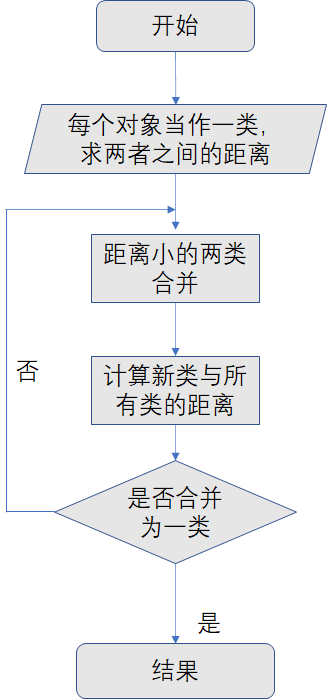
\includegraphics[width=0.4\textwidth,height=0.72\textwidth]{img/Clustering.png} % 图片相对位置
	\caption{Clustering}
	\label{fig:figure 2} % 图片标签
	\end{figure}



综合上三表数据,类别1的企业大部分为2020年依然盈利或者不盈不亏;
平均$Void_{ij}$较小,$Trade_{ij}$大部分为正且数值较大,说明疫情对于这些企业的影响较小,供求关系稳定甚至仍有盈利;
类别2 的企业大部分为亏损,特征值$Void_{ij}$和$Trade_{ij}$都比类别1要表现更差;类别3的企业有4个,全部为高风险的企业。

根据以上聚类出的三类行业的表现,本文设置其对应的风险乘数为:

$Q_1=1$,$Q_2=1.5$,$Q_3=2$,
	 
\subsubsection{}
附件2中及本文将企业依据信誉评级分为4 类,在建立模型的过程中根据疫情对企业的影响将企业分为3类,
同时将违约和D 级企业不放贷款且聚类结果的类别3全为D级企业。将数据分为6类,
根据聚类结果建立一个新的评价分级体系,记为$A_1$,$A_2$,$B_1$,$B_2$,$C_1$,$C_2$,。
将风险乘数$Q_i$加入信贷目标规划模型,调整企业风险,建立调整后的多目标规划模型如下:
\begin{equation}
	\min \sum_{n = 1}^{3}\sum_{m}C_i(1+Q_m)\overline{\sigma }_n P_n (1+I_m)+I_n P_n \frac{C_n Lost(I_n)}{1-Lost(I_n)}-C_n I_n P_n   
\end{equation}

限制条件为:
\[\left\{\begin{array}{lllll}
	\sum_{n = 1}^{6}C_n  P_n = 10^7 \\
	0.04 \le I_1 \le 0.15\\
	0.058 \le I_2 \le 0.15\\
	0.076 \le I_3 \le 0.15\\
	0.094 \le I_4 \le 0.15\\
	0.112 \le I_5 \le 0.15\\
	0.13 \le I_6 \le 0.15\\
	10^5 \le P_1 \le 10^6\\
	10^5 \le P_2 \le 8.5*10^5\\
	10^5 \le P_3 \le 7*10^5\\
	10^5 \le P_4 \le 5.5*10^5\\
	10^5 \le P_5 \le 4*10^5\\
	10^5 \le P_6 \le 2.5*10^5\\

	\end{array}\right. \]

计算得出如下结果:

\begin{center}
	\centering
	\begin{tabular}{||c c c c ||}
		
		\hline
		企业类别 & 数量 & 利率 & 金额        \\ [0.5ex]
		\hline
		$A_1$   & 54     & 7.60$\%$ & 999988  \\
		\hline
		$A_2$   & 9     & 6.25$\%$ & 849863  \\
		\hline
		$B_1$   & 82     & 11.20$\%$ & 317698  \\
		\hline
		$B_2$   & 21     & 9.40$\%$ & 100017  \\
		\hline
		$C_1$   & 87     & 11.20$\%$ & 100002  \\
		\hline
		$C_2$   & 15     & 13.00$\%$ & 100006  \\
		\hline
	\end{tabular}
\end{center}


\section{模型分析}
\subsection{优点}

1、综合考量了企业自身能力和多方因素,从而提取了具有相特征性的特征值数据,较为全面的考虑了问题。

2、使用了多种算法和模型,采用强分类器,效果良好,以及$Voting$集成算法,所得出的结果准确较高,
训练求解的结果可信度同样也很高。

3、考虑信贷策略时,综合考虑了多目标规划,在所提取特征值的基础上,加入了风险系数以及信誉等级
的分类,使得模型更加贴合实际情况。

4、采用的聚类模型在处理突发因素所带来的影响时,得出的轮廓系数接近1,聚类效果好。

\subsection{缺点}
1、数据不够充分,考虑疫情对评估影响时只采用了两年分别四个月的数据,数据不够充分,说服性不足。

2、考虑突发情况时没有充分考虑对企业大类的影响,只考虑了新冠疫情,因素不够多。

3、特征值提取过多,且有的特征值其特征性不明显,作用不大。

4、未对企业进行行业的分类,考虑行业受因素的影响以及总体社会的受干扰因素。

\subsection{改进}
1、可以尝试采用修正因子量化分析的方法来对整体企业进行新的风险评估。

2、可以将企业依据行业进行分类,更好的考虑行业的整体受突发因素影响。


% %引用
% \clearpage
% \bibliographystyle{plain}
% \bibliography{ref}%ref指向自己创建的ref.bib
% % IoU\cite{zheng2020distance}
% \clearpage

% \section{附录}
% \subsection{代码}

% \lstset{language=python}
% \begin{lstlisting}
% 	import time
% 	import numpy as np
% 	import pandas as pd
% 	import matplotlib.pyplot as plt

		
% \end{lstlisting}

\end{document}
